\documentclass[a4paper]{article}
\usepackage[a4paper,margin=0mm]{geometry}
\usepackage{fontspec}
\usepackage{unicode-math}
\usepackage{tikz}
\usepackage[table]{xcolor}
\usepackage[absolute]{textpos}
\usepackage{enumitem}
\usepackage{array}
\usepackage{multirow}

\setmainfont{Libertinus Serif}
\setsansfont{Libertinus Sans}
\setmathfont{Libertinus Math}
\newfontfamily\trackedsans{Libertinus Sans}[LetterSpace=8.0]

\definecolor{accent}{HTML}{F46530}
\definecolor{badge}{HTML}{FFBDA5}
\definecolor{ink}{HTML}{2A2E30}

\setlength{\TPHorizModule}{1mm}
\setlength{\TPVertModule}{1mm}
\setlength{\parindent}{0pt}
\pagestyle{empty}

\newcommand{\LCOL}{16mm}
\newcommand{\RCOL}{111mm}
\newcommand{\COLW}{83mm}

\newcommand{\topicheader}[2]{%
\begin{textblock*}{194mm}(16mm,10mm)
\begin{tikzpicture}
\node[fill=accent,text=white,font=\sffamily\bfseries\fontsize{13}{13}\selectfont,
      minimum width=9mm,minimum height=9mm,inner sep=0pt] at (4.5mm,-4.5mm) {#1};
\node[font=\sffamily\bfseries\fontsize{15}{16}\selectfont,text=ink,anchor=west] at (12mm,-4.5mm) {#2};
\end{tikzpicture}
\end{textblock*}
\begin{textblock*}{194mm}(16mm,22.5mm)

\begin{tikzpicture}
\fill[accent] (0,0) rectangle (194mm,0.5mm);
\end{tikzpicture}
\end{textblock*}
}

\newcommand{\pagefooter}[1]{%
\begin{textblock*}{194mm}(8mm,286.41mm)
  
\begin{tikzpicture}
    \fill[accent] (0,0) rectangle (194mm,0.6mm);
  \end{tikzpicture}
\end{textblock*}
\begin{textblock*}{63.59mm}(8mm,288.27mm)
  {\sffamily\bfseries\color{accent}\fontsize{13}{16}\selectfont SAT 1200+}
\end{textblock*}
\begin{textblock*}{10mm}(188mm,288.27mm)
  \centering{\sffamily\color{accent}\fontsize{14}{16}\selectfont #1}
\end{textblock*}
}

\newcommand{\colrule}[2]{%
\begin{textblock*}{1mm}(105mm,#1mm)
\begin{tikzpicture}
\draw[black!65,line width=0.5pt] (0,0) -- (0,#2mm);
\end{tikzpicture}
\end{textblock*}
}

\newcommand{\setkicker}[2]{%
{\sffamily\bfseries\fontsize{12}{14}\selectfont #1.}\ {\itshape\fontsize{11}{14}\selectfont\color{black!75} #2}\par\vspace{2mm}%
}

\setlength{\fboxsep}{1.4pt}
\setlength{\fboxrule}{0.5pt}
\newcommand{\pnum}[1]{\fcolorbox{ink}{white}{\sffamily\bfseries\fontsize{8}{8}\selectfont #1}~}

\newcommand{\qrbox}[1]{%
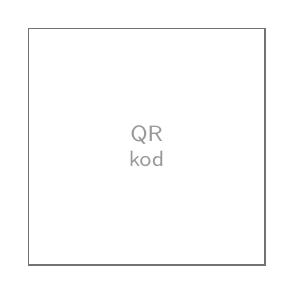
\begin{tikzpicture}
\draw[black!55,line width=0.6pt] (0,0) rectangle (30mm,30mm);
\node[black!40,font=\sffamily\fontsize{8}{9}\selectfont,align=center] at (15mm,15mm) {QR\\kod};
\end{tikzpicture}\\[1.5mm]
{\sffamily\fontsize{9}{11}\selectfont\color{black!70} #1}%
}

\arrayrulecolor{accent}
\setlength{\arrayrulewidth}{0.7pt}
\renewcommand{\arraystretch}{1.35}
\newcommand{\anstitle}[1]{{\sffamily\bfseries\color{accent}\fontsize{11}{13}\selectfont #1}\\[1.3mm]}

\begin{document}

% ================= PAGE 1: Set 1 | Set 2 =================
\topicheader{3}{O'nli kasrlar va foizlar}
\pagefooter{1}
\colrule{32}{238}
\mbox{}%

\begin{textblock*}{\COLW}(\LCOL,32mm)
{\fontsize{12}{15}\selectfont
\setkicker{1-to'plam}{O'nli kasrlarni qo'shish va ayirish: vergulni tekislashni unutmang.}

\noindent\pnum{1} $3.7+2.45=$\\[22mm]
\noindent\pnum{2} $12.6-4.75=$\\[22mm]
\noindent\pnum{3} $0.8+0.09=$\\[22mm]
\noindent\pnum{4} $15-3.25=$\\[22mm]
\noindent\pnum{5} $2.05+1.95=$\\[22mm]
\noindent\pnum{6} $100-0.4=$\\[22mm]
\noindent\pnum{7} $0.125+0.875=$\\[22mm]
\noindent\pnum{8} $7.3-2.08=$
}
\end{textblock*}

\begin{textblock*}{\COLW}(\RCOL,32mm)
{\fontsize{12}{15}\selectfont
\setkicker{2-to'plam}{O'nli kasrlarni ko'paytirish va bo'lish -- kasr xonalarini to'g'ri sanang.}

\noindent\pnum{1} $0.3\times0.4=$\\[22mm]
\noindent\pnum{2} $2.5\times1.2=$\\[22mm]
\noindent\pnum{3} $0.06\times5=$\\[22mm]
\noindent\pnum{4} $1.44\div1.2=$\\[22mm]
\noindent\pnum{5} $0.5\times0.5=$\\[22mm]
\noindent\pnum{6} $7.2\div0.4=$\\[22mm]
\noindent\pnum{7} $0.02\times0.03=$\\[22mm]
\noindent\pnum{8} $9.6\div2.4=$
}
\end{textblock*}

\clearpage

% ================= PAGE 2: Set 3 | Set 4 =================
\topicheader{3}{O'nli kasrlar va foizlar}
\pagefooter{2}
\colrule{32}{238}
\mbox{}%

\begin{textblock*}{\COLW}(\LCOL,32mm)
{\fontsize{12}{15}\selectfont
\setkicker{3-to'plam}{O'nli kasr $\leftrightarrow$ oddiy kasr almashtirish.}

\noindent\pnum{1} $0.5$ ni oddiy kasrga aylantiring.\\[20mm]
\noindent\pnum{2} $0.25$ ni oddiy kasrga aylantiring.\\[20mm]
\noindent\pnum{3} $0.75$ ni oddiy kasrga aylantiring.\\[20mm]
\noindent\pnum{4} $0.2$ ni oddiy kasrga aylantiring.\\[20mm]
\noindent\pnum{5} $\dfrac{3}{4}$ ni o'nli kasrga aylantiring.\\[20mm]
\noindent\pnum{6} $\dfrac{1}{8}$ ni o'nli kasrga aylantiring.\\[20mm]
\noindent\pnum{7} $\dfrac{7}{10}$ ni o'nli kasrga aylantiring.\\[20mm]
\noindent\pnum{8} $0.125$ ni oddiy kasrga aylantiring.
}
\end{textblock*}

\begin{textblock*}{\COLW}(\RCOL,32mm)
{\fontsize{12}{15}\selectfont
\setkicker{4-to'plam}{Foiz $\leftrightarrow$ o'nli kasr almashtirish -- $100\%$ dan katta va $1\%$ dan kichik holatlarni ham o'z ichiga oladi.}

\noindent\pnum{1} $45\%$ ni o'nli kasrga aylantiring.\\[18mm]
\noindent\pnum{2} $7\%$ ni o'nli kasrga aylantiring.\\[18mm]
\noindent\pnum{3} $150\%$ ni o'nli kasrga aylantiring.\\[18mm]
\noindent\pnum{4} $0.5\%$ ni o'nli kasrga aylantiring.\\[18mm]
\noindent\pnum{5} $0.6$ ni foizga aylantiring.\\[18mm]
\noindent\pnum{6} $1.25$ ni foizga aylantiring.\\[18mm]
\noindent\pnum{7} $0.03$ ni foizga aylantiring.\\[18mm]
\noindent\pnum{8} $2$ ni foizga aylantiring.
}
\end{textblock*}

\clearpage

% ================= PAGE 3: Set 5 | Set 6 (spot the error) =================
\topicheader{3}{O'nli kasrlar va foizlar}
\pagefooter{3}
\colrule{32}{238}
\mbox{}%

\begin{textblock*}{\COLW}(\LCOL,32mm)
{\fontsize{12}{15}\selectfont
\setkicker{5-to'plam}{Foiz $\leftrightarrow$ oddiy kasr, va sonning foizini topish.}

\noindent\pnum{1} $80$ ning $25\%$ i qanchaga teng?\\[20mm]
\noindent\pnum{2} $150$ ning $10\%$ i qanchaga teng?\\[20mm]
\noindent\pnum{3} $45$ ning $60\%$ i qanchaga teng?\\[20mm]
\noindent\pnum{4} $\dfrac{1}{4}$ ni foizga aylantiring.\\[20mm]
\noindent\pnum{5} $\dfrac{3}{5}$ ni foizga aylantiring.\\[20mm]
\noindent\pnum{6} $150\%$ ni oddiy kasrga aylantiring.\\[20mm]
\noindent\pnum{7} $50$ ning $12\%$ i qanchaga teng?\\[20mm]
\noindent\pnum{8} $20$ ning $90\%$ i qanchaga teng?
}
\end{textblock*}

\begin{textblock*}{\COLW}(\RCOL,32mm)
{\fontsize{11}{14}\selectfont
\setkicker{6-to'plam}{Xatoni toping -- buzilgan qadamni ayting, to'g'ri javobni bering.}

\noindent\pnum{1} $80$ ning $45\%$ ini hisoblashda ko'rsatilgan yechimda xato bor:\\[1mm]
\hspace*{7mm}\textit{``$45\times80=3600$, demak javob $3600$.''}\\[2mm]
\hspace*{7mm}Xato va to'g'ri javob: \makebox[52mm]{\dotfill}\\[8mm]

\noindent\pnum{2} $3.7+2.45$ ni hisoblashda ko'rsatilgan yechimda xato bor:\\[1mm]
\hspace*{7mm}\textit{``Vergulni tekislamasdan qo'shib, $3.7+2.45=2.82$ deb topilgan.''}\\[2mm]
\hspace*{7mm}Xato va to'g'ri javob: \makebox[52mm]{\dotfill}\\[8mm]

\noindent\pnum{3} $1.44\div1.2$ ni hisoblashda ko'rsatilgan yechimda xato bor:\\[1mm]
\hspace*{7mm}\textit{``Kasr xonalarini noto'g'ri sanab, $1.44\div1.2=0.12$ deb topilgan.''}\\[2mm]
\hspace*{7mm}Xato va to'g'ri javob: \makebox[52mm]{\dotfill}\\[8mm]

\noindent\pnum{4} $0.2$ ni oddiy kasrga aylantirishda ko'rsatilgan yechimda xato bor:\\[1mm]
\hspace*{7mm}\textit{``$0.2$ dagi raqam yuzdan bir xonasida deb o'ylab, $\frac{2}{100}=\frac{1}{50}$ deb topilgan.''}\\[2mm]
\hspace*{7mm}Xato va to'g'ri javob: \makebox[52mm]{\dotfill}\\[8mm]

\noindent\pnum{5} $150\%$ ni o'nli kasrga aylantirishda ko'rsatilgan yechimda xato bor:\\[1mm]
\hspace*{7mm}\textit{``Vergul faqat bir xona chapga surilib, $150\%=15$ deb topilgan.''}\\[2mm]
\hspace*{7mm}Xato va to'g'ri javob: \makebox[52mm]{\dotfill}
}
\end{textblock*}

\clearpage

% ================= PAGE 4: Set 7 (bonus) -- own page =================
\topicheader{3}{O'nli kasrlar va foizlar}
\pagefooter{4}
\colrule{32}{238}
\mbox{}%

\begin{textblock*}{\COLW}(\LCOL,32mm)
{\fontsize{12}{15}\selectfont
\setkicker{7-to'plam}{Bonus / qiyin -- aralash almashtirishlar, har biriga taxminan 90 soniya.}

\noindent\pnum{1} $0.8$ ning $35\%$ ini toping, so'ngra natijani $100$ ga ko'paytiring.\\[26mm]
\noindent\pnum{2} $\dfrac{3}{8}$ ni foizga aylantiring.\\[26mm]
\noindent\pnum{3} $0.6$ ning necha foizi $0.3$ ga teng?\\[26mm]
\noindent\pnum{4} $1.5$ ni foizga va oddiy kasrga aylantiring.\\[26mm]
\noindent\pnum{5} $(0.25+0.5)$ yig'indisining $40\%$ ini toping.
}
\end{textblock*}

\clearpage

% ================= PAGE 5: Javoblar -- single unified answer table =================
\topicheader{3}{O'nli kasrlar va foizlar}
\pagefooter{5}
\mbox{}%

\begin{textblock*}{194mm}(16mm,30mm)
{\bfseries\itshape\color{accent}\fontsize{19}{21}\selectfont\centering Javoblar\par}
\end{textblock*}

\begin{textblock*}{194mm}(16mm,44mm)
{\fontsize{10}{12.5}\selectfont
\centering
\renewcommand{\arraystretch}{1.3}
\begin{tabular}{|>{\centering\arraybackslash}p{26mm}|>{\centering\arraybackslash}p{10mm}|>{\centering\arraybackslash}p{28mm}|>{\centering\arraybackslash}p{10mm}|>{\centering\arraybackslash}p{28mm}|}
\hline
\rowcolor{badge!55}\textbf{To'plam} & \textbf{\#} & \textbf{Javob} & \textbf{\#} & \textbf{Javob}\\
\hline
\multirow{4}{26mm}{\centering 1-to'plam} & 1 & 6.15 & 2 & 7.85\\\cline{2-5}
 & 3 & 0.89 & 4 & 11.75\\\cline{2-5}
 & 5 & 4 & 6 & 99.6\\\cline{2-5}
 & 7 & 1 & 8 & 5.22\\\hline
\multirow{4}{26mm}{\centering 2-to'plam} & 1 & 0.12 & 2 & 3\\\cline{2-5}
 & 3 & 0.3 & 4 & 1.2\\\cline{2-5}
 & 5 & 0.25 & 6 & 18\\\cline{2-5}
 & 7 & 0.0006 & 8 & 4\\\hline
\multirow{4}{26mm}{\centering 3-to'plam} & 1 & 1/2 & 2 & 1/4\\\cline{2-5}
 & 3 & 3/4 & 4 & 1/5\\\cline{2-5}
 & 5 & 0.75 & 6 & 0.125\\\cline{2-5}
 & 7 & 0.7 & 8 & 1/8\\\hline
\multirow{4}{26mm}{\centering 4-to'plam} & 1 & 0.45 & 2 & 0.07\\\cline{2-5}
 & 3 & 1.5 & 4 & 0.005\\\cline{2-5}
 & 5 & 60\% & 6 & 125\%\\\cline{2-5}
 & 7 & 3\% & 8 & 200\%\\\hline
\multirow{4}{26mm}{\centering 5-to'plam} & 1 & 20 & 2 & 15\\\cline{2-5}
 & 3 & 27 & 4 & 25\%\\\cline{2-5}
 & 5 & 60\% & 6 & 3/2\\\cline{2-5}
 & 7 & 6 & 8 & 18\\\hline
\multirow{3}{26mm}{\centering 7-to'plam} & 1 & 28 & 2 & 37.5\%\\\cline{2-5}
 & 3 & 50\% & 4 & 150\%, 3/2\\\cline{2-5}
 & 5 & 0.3 & -- & --\\\hline
\multirow{5}{26mm}{\centering 6-to'plam} & \multicolumn{4}{p{76mm}|}{1.\ Foiz to'g'ridan-to'g'ri ko'paytirilgan, o'nli kasrga aylantirilmagan. To'g'ri: $45\%=0.45$, so'ng $0.45\times80=36$.}\\\cline{2-5}
 & \multicolumn{4}{p{76mm}|}{2.\ Vergullar tekislanmagan. To'g'ri: $3.70+2.45=6.15$.}\\\cline{2-5}
 & \multicolumn{4}{p{76mm}|}{3.\ Kasr xonalari noto'g'ri sanalgan. To'g'ri: $1.44\div1.2=1.2$.}\\\cline{2-5}
 & \multicolumn{4}{p{76mm}|}{4.\ Raqamning xonasi noto'g'ri aniqlangan (yuzdan emas, o'ndan). To'g'ri: $0.2=\frac{2}{10}=\frac{1}{5}$.}\\\cline{2-5}
 & \multicolumn{4}{p{76mm}|}{5.\ Vergul bir xona o'rniga ikki xona chapga surilishi kerak edi. To'g'ri: $150\%=1.50=1.5$.}\\\hline
\end{tabular}
}
\end{textblock*}

\begin{textblock*}{194mm}(16mm,240mm)
\centering
{\sffamily\fontsize{9.5}{11.5}\selectfont\color{black!70} Video yechimlar va qo'shimcha testlar uchun quyidagi QR kodlarni skanerlang:}\\[4mm]
\begin{minipage}[t]{32mm}\centering\qrbox{YouTube}\end{minipage}%
\hspace{16mm}%
\begin{minipage}[t]{32mm}\centering\qrbox{Telegram}\end{minipage}
\end{textblock*}

\end{document}
